\section{Data}
\label{sec:data}

% What data did you use in your project? How was this data created What preprocessing did you do (if any), and why?

The dataset used in this project consists of about 14k medical abstracts describing different patient conditions, labeled in five different categories: 1. neoplasms, 2. digestive system diseases, 3. nervous system diseases, 4. cardiovascular diseases, and 5. general pathological conditions. The data was compiled by Schopf et al. in conjunction with the paper \textit{“Evaluating Unsupervised Text Classification: Zero-Shot and Similarity-Based Approaches”} \cite{Schopf2022EvaluatingApproaches}, and pre-divided into training and testing data. 

The final data used was then a pre-processed version of the original dataset. First, the test data was reduced to 50\% of the original size. This was done since the later methods makes use of the OpenAI API\footnote{https://platform.openai.com/overview} to access the OpenAI model GPT-3.5 Turbo\footnote{https://platform.openai.com/docs/models/gpt-3-5-turbo}, which is not free of charge. Using too large a dataset would increase the total cost of the project, which was preferred to be kept as low as possible. Reducing the dataset was done using scikit-learn's\footnote{https://scikit-learn.org/stable/} (a common python package for data analysis) built-in function \textit{“train\_test\_split”}, using the condition label as \textit{“stratify”} to ensure the original class balance.

Second, looking at the structure of the training data, one could see that the classes were quite imbalanced. Since this could pose a problem for statistical methods for classification, the data was balanced by undersampling to the minority class. This of course also reduced the size of the training data set. Figure \ref{fig:pre-undersample} and \ref{fig:post-undersample} shows the difference in the data structure before and after undersampling, respectively. Final training data contained 1200 examples of each class. No processing changing the balance of the test data was done.

\begin{figure}[ht]
    \centering
    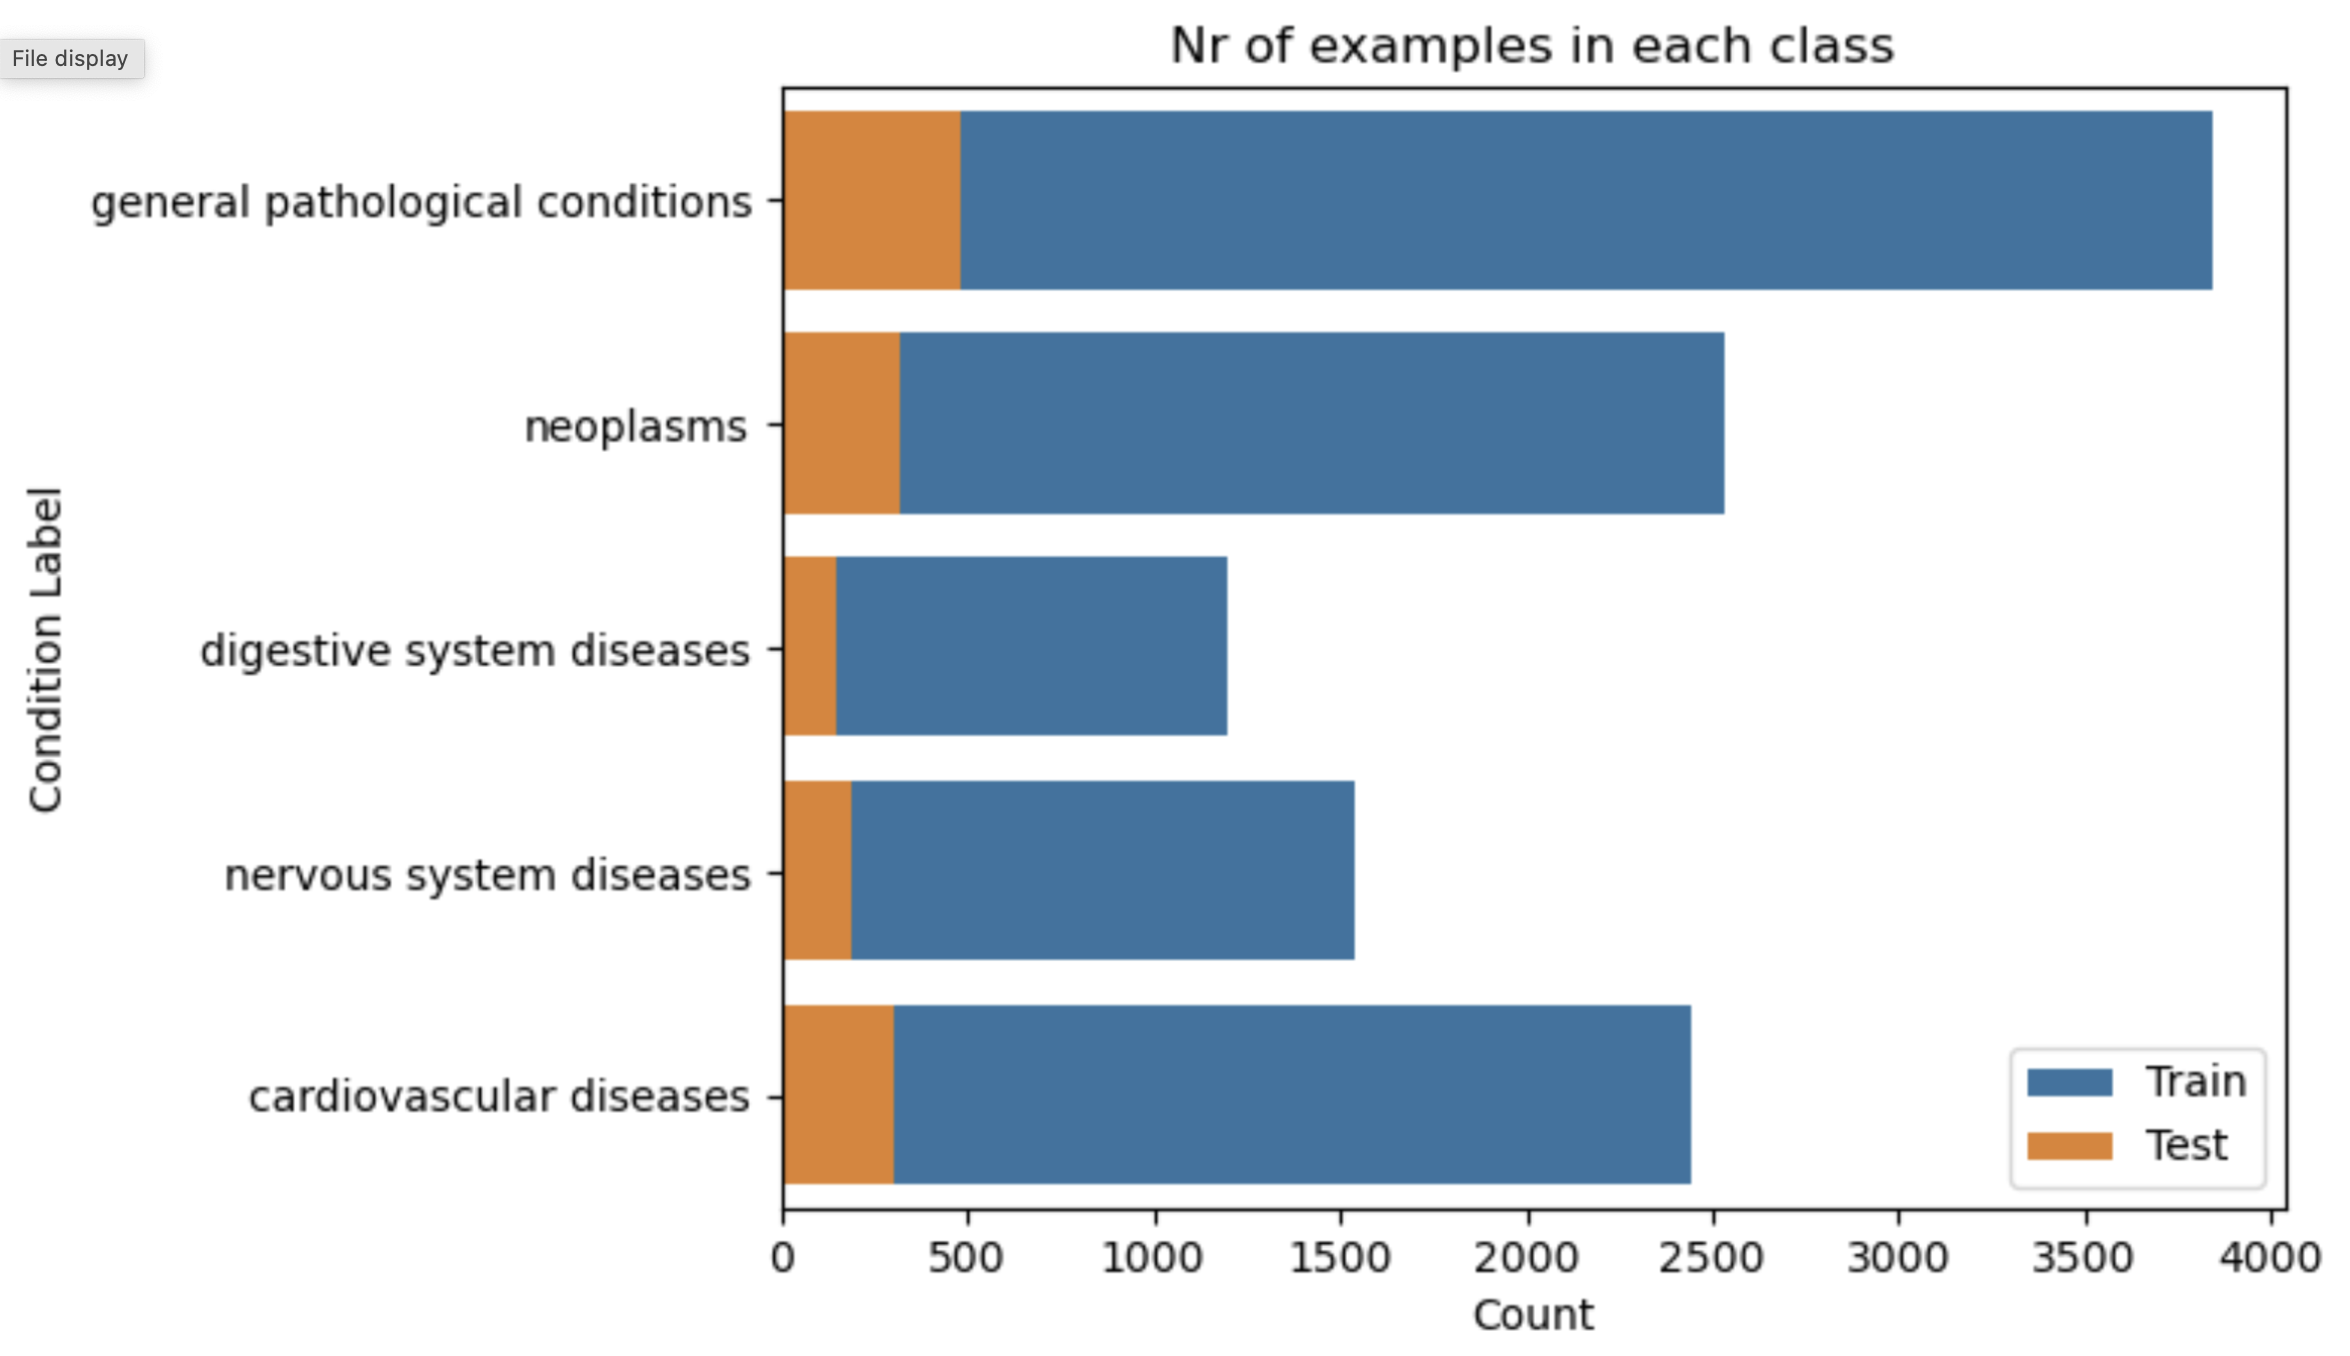
\includegraphics[width=\columnwidth]{report/figures/data-pre-undersample.png} % Replace 'example-image' with your image file name
    \caption{Structure of data pre undersample.}
    \label{fig:pre-undersample}
\end{figure}
\vspace{-1em}
\begin{figure}[ht]
    \centering
    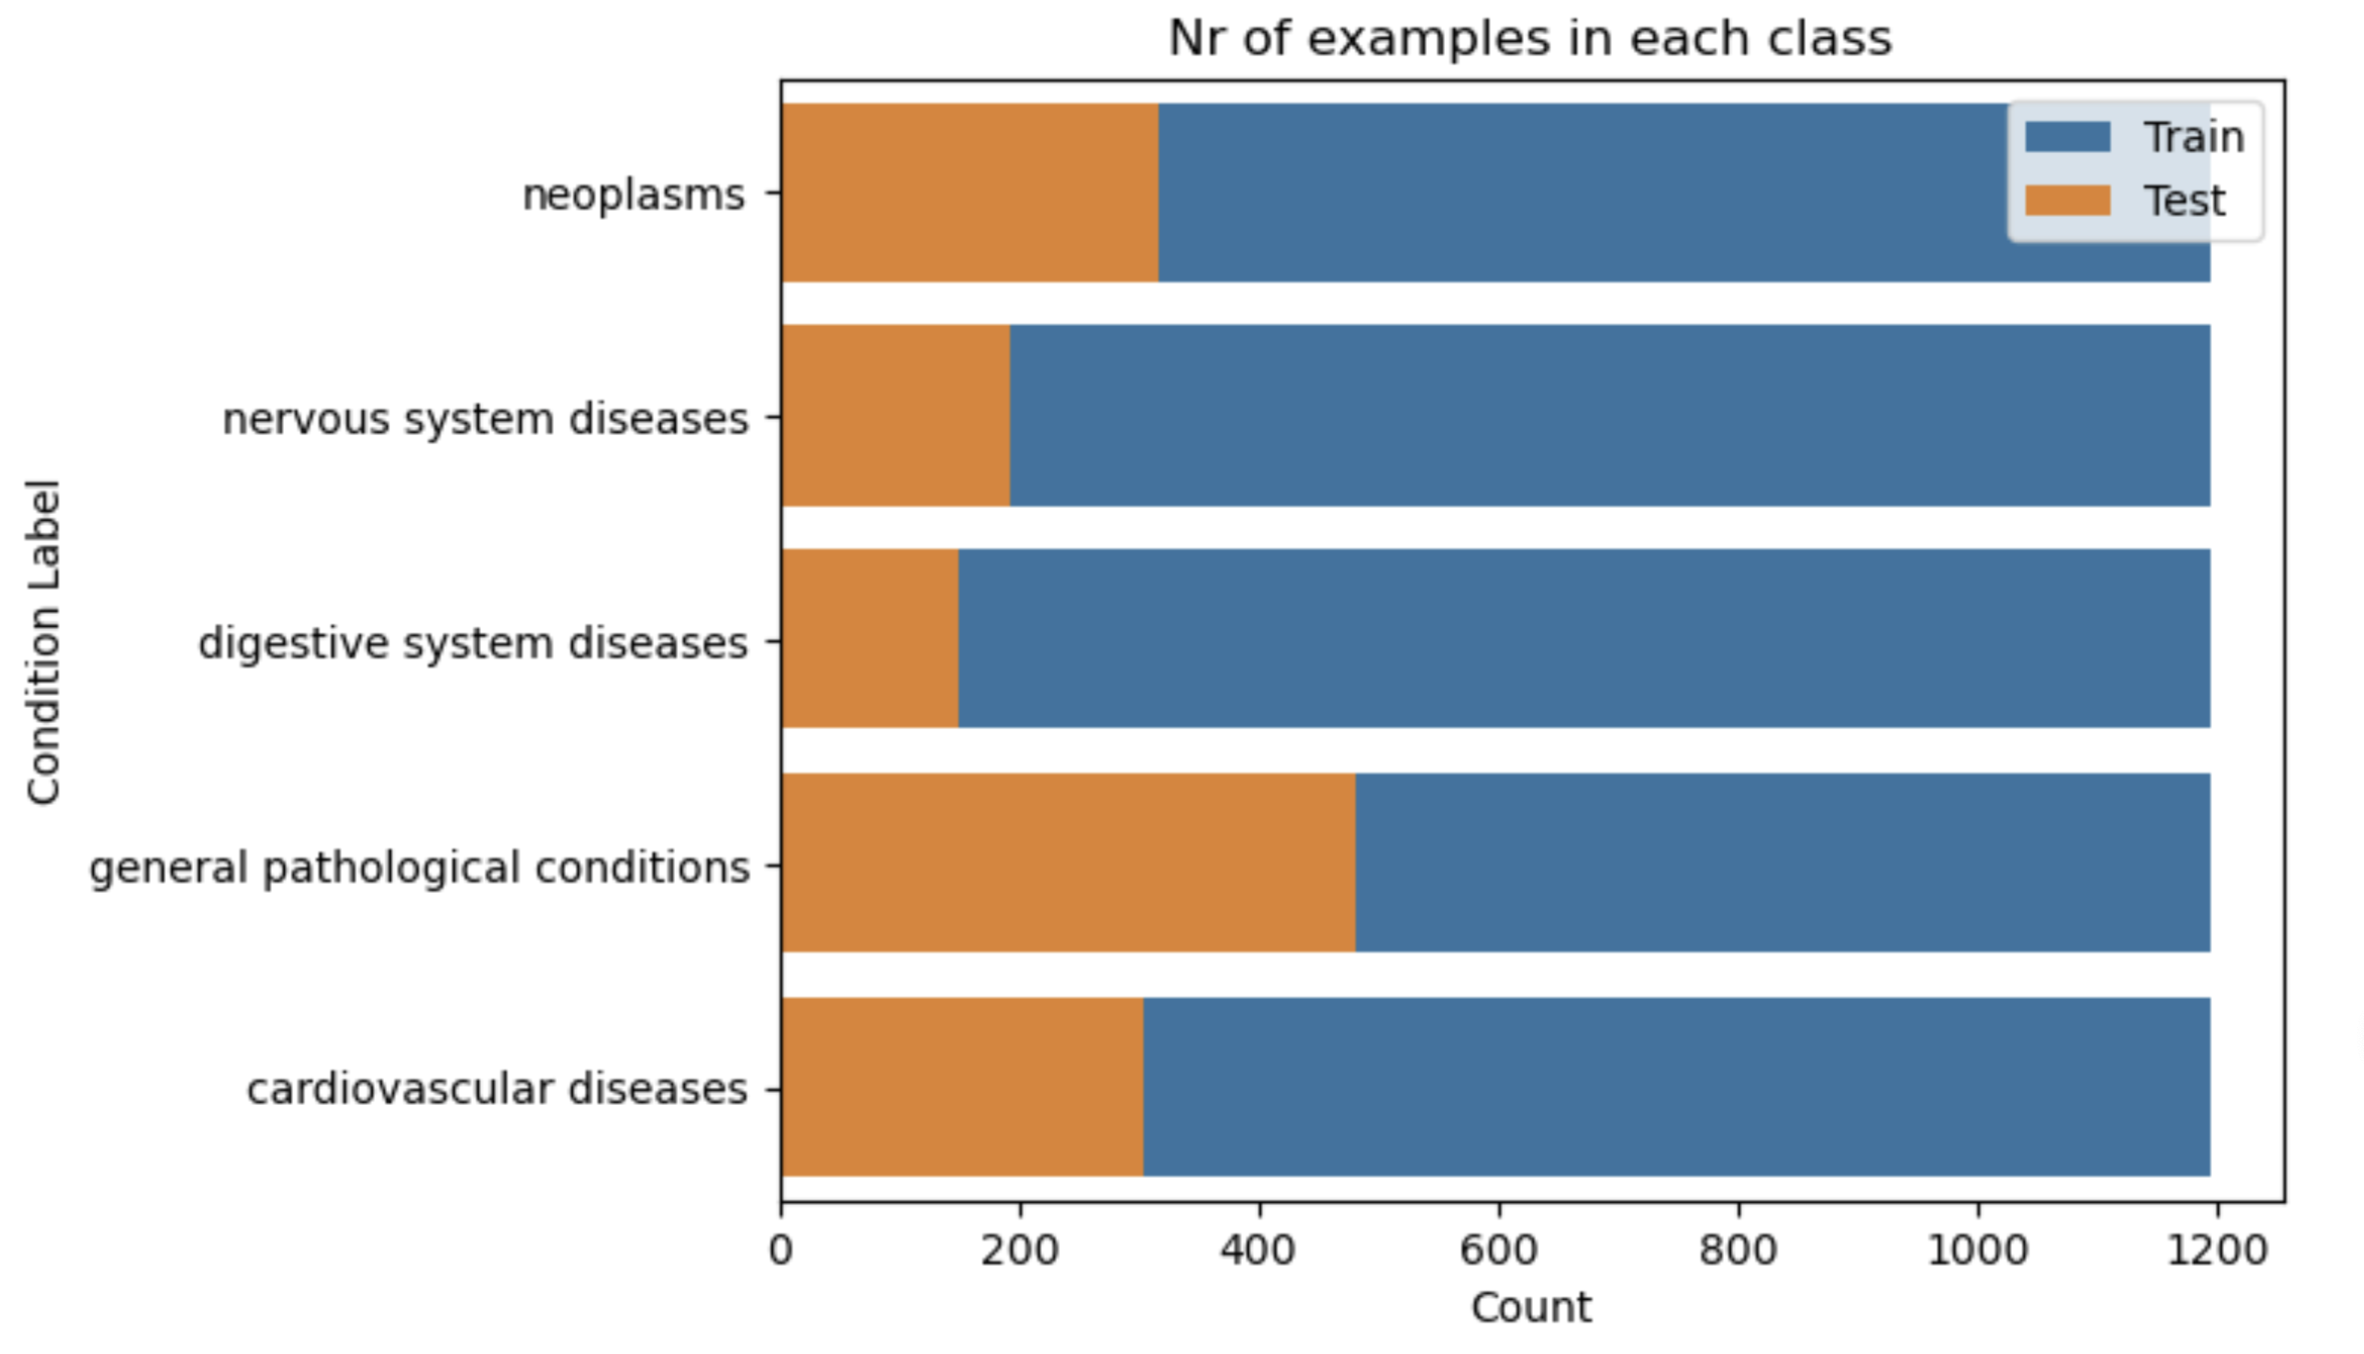
\includegraphics[width=\columnwidth]{report/figures/data-post-undersample.png} % Replace 'example-image' with your image file name
    \caption{Structure of data post undersample.}
    \label{fig:post-undersample}
\end{figure}